% ===================================================================
% Arquivo: capitulos/parte-III-pilares/cap-06-retropropagacao-e-gradiente.tex
% ===================================================================

\chapter{O Algoritmo da Repropropagação e Os Otimizadores Baseados em Gradiente}
\label{cap:retropropagacao-gradiente}

\begin{flushright}
\textit{A filosofia de vida do gradiente descendente: 'Pra lá é pra baixo? É. Então eu vou pra lá.'} \\
--- A Sabedoria do Algoritmo
\end{flushright}

% ===================================================================
% Resumo do capítulo
% ===================================================================

Cada rede neural é composta de diferentes partes, uma rede feedforward é composta de camadas densas, que por sua vez são compostas por um conjunto de neurônios. Uma rede convolucional, possui camadas de achatamento, camadas de pooling e camadas convolucionais, que possuem kernels muitas vezes inteligêntes que aprendem conforme o o treino a reconhecer diferentes padrões em imagens. Já uma rede recorrente, possui camadas com neurônios recorrentes, que buscam reconhecer padrões em diferentes tipos de séries, a fim de que seja por exemplo, possível prever qual será o valor de ação de uma marca x no dia 27 de setembro de 2025.

O que não falta em uma rede neural são parâmetros, eles estão por todos os lados. Agora imagine que você está encarregado de criar uma rede convolucional para reconhecer imagens de cães e gatos e precisa de forma manual ajustar todos, o pesos das camadas densas junto com o seus vieses, além de ter que atualizar os valores de um kernel presente na primeira camada convolucional.

Certamente isso é impossível de ser feito, uma rede como essa pode ter milhares e até milhões de parâmetros. Por isso, uma das formas de contornar esse problema, e, deixar para que o computador faça as suas atualiações é a retropropagação. Ela caminha junto com o método do gradiente para que todas essas atualições sejam feitas de forma automática, e com uma maior garantia que ela será eficáz, uma vez que estará se baseando em como o erro do modelo que está sendo treinado é medido.

Esse capítulo se inicia explicando o conceito do método do gradiente, e como ele foi o ponto de partida para que a os pesquisadores pudessem criar a retropropagação. Contudo, essa otimização com o tempo passou a ser demorada, e assim, novos métodos surgiram, como o gradiente descendente com momento. Conforme o poder compuaticional foi aumento, outros métodos mais modernos também surgiram, apresentando conceitos novos, como múltiplas taxas de aprendizado, como o AdaGrad, de forma que características menos frequêntes possuíssem uma taxa de aprendado maior, indicando que o modelo que estava sendo criado seria mais sensível à essas propriedades, e com isso, ele pudesse "tomar nota" quando uma informação assim aparecesse.

% ===================================================================
% Método do Gradiente Descendente
% ===================================================================

\section{O Método do Gradiente Descendente: A Inspiração de Todos}

O Método do Gradiente faz parte de uma série de métodos numéricos que possuem como função otimizar diferentes funções. Métodos dessa forma veem sendo estudados a séculos, um exemplo disso é o trabalho \textit{M{\'e}thode g{\'e}n{\'e}rale pour la r{\'e}solution des syst{\`e}mes d'{\'e}quations simultan{\'e}es} (Método geral para resolução de sistemas de equações simultâneos em portguês) do matemático francês do século XVIII \textcite{CauchyMetodoDoGradiente}, em que o autor apresenta um método que pode ser considerado um precursor para o método do gradiente atual.

Nesse texto, o autor apresenta uma forma de minimizar uma função de múltiplas variáveis ($u=f(x,y,z)$) que não assume valores negativos, para fazer isso, ele faz uso do cálculo de derivadas parciais dessa função de cada um dos seus componentes ($D_x u, D_y u, D_z u$), em seguida, ele realiza um passo de atualização, de forma que os os valores de cada uma das variáveis sejam ligeiramente incrementados por valores ($\alpha, \beta, \gamma$) \parencite{CauchyMetodoDoGradiente}. Um ponto importante destacado por \textcite{CauchyMetodoDoGradiente} é de que esses incrementos devem ser proporcionais ao negativo das suas respectivas derivadas parciais, ele descreve que esse processo de calcular as derivadas e fazer pequenos incrementos deve ser feito de forma iterativa, assim, calculá-se as derivadas, faz-se os incrementos, e o passo é repetido até convergir para o valor mínimo de $u$.

Esse trabalho explica bem como aplicar o método do gradiente para se calcular mínimos de funções, mas para facilitar o entendimento do leitor, em seguida está um exemplo ilutrativo explicando o funcionamento dessa ferramenta.

\subsection{Exemplo Ilustrativo: Cadeia de Montanhas}

Imagine que você adora aventuras, e por isso, decidiu fazer uma trilha em uma floresta que fica em uma cadeia de montanhas que podem ser escaladas. Então, você teve a incrivel ideia de ir para o menor ponto dessa cadeia de montanhas, pois, no guia que você estava seguindo, falava que lá havia um lago com uma água cristalina, perfeito para tirar fotos.

Para chegar até esse lago, você conta com uma bússula um tanto quanto diferente, ao invés dela apontar para o norte como uma bússola comum, ela aponta para a direção do lugar com menor altitude de uma região. Isso é perfeito para o que você precisa, pois ela irá apontar justamente para o lago de você quer ir.

Com isso em mente, você criou um plano de como irá chegar a esse lago, ele é método que segue dois passos diferentes, sendo eles:

\begin{enumerate}
    \item Olha na bússola qual a direção ela está apontando;
    \item Anda um metro na direção apontada pela bússola.
\end{enumerate}

Você chegou na conclusão que se seguir essa estratégia repetidas vezes, em algum momento, você inevitavelmente irá chegar no lago que está querendo tirar as suas fotos.

Na matemática, existe um método semelhante a este, que busca com base em uma bússola (chamada de vetor gradiente), encontrar um ponto de mínimo de um determinado lugar (neste caso, uma função composta por múltiplas variáveis). Esse é o método do gradiente, ele é ponto central desse capítulo, pois, ele (e suas variações) junto com o algortimo da retroprogação são algumas das principais ferramentas que colaboram para que os modelos de aprendizado de máquina possam aprender com os seus erros e com isso se tornarem melhores a cada iteração.

\subsection{O Método em Si}

A vantagem do método do gradiente é que ele é uma ferramenta matemática, e por isso pode ser representado utilizando notações mais formais e de forma enxuta. As notações utilizadas por Cauchy são diferentes das que são utilizadas hoje em dia, mas o seu significado não muda. Em \textit{Deep Learning}, \textcite{DeepLearningBook} explicam essa ferramenta através da equação \ref{eq:metodo-do-gradiente} que deve ser repetida por múltiplos passos até o modelo convergir, ou seja, encontrar o ponto de mínimo da função estudada.

\begin{equacaodestaque}{Método do Gradiente Descendente}
    x = x_0 - \epsilon \nabla f(x_0)
    \label{eq:metodo-do-gradiente}
\end{equacaodestaque}

Em que:

\begin{itemize}
    \item $x'$: representa as coordenadas do próximo ponto;
    \item $x$: representa as coordernadas do ponto atual;
    \item $\epsilon$: representa o tamanho do passo, também chamado de taxa de aprendizado;
    \item $\nabla f(x)$: representa o vetor gradiente calculado na posição do ponto atual ($x$) para função que se deseja otimizar.
\end{itemize}

Note que assim como no método proposto por Cauchy, é pego como base o inverso do vetor gradiente. Isso ocorre pois o vetor gradiente é um vetor especial que tem como principal propriedade apontar para a direção de maior crescimento de uma função no ponto que está sendo calculada. Mas no método, o objetivo não é encontrar o ponto que irá gerar os maiores valores da função, e sim o contrário. Por isso, é tomado inverso do vetor gradiente, que, dessa forma, estará então apontando para a direção de menor crescimento de uma função.

Um ponto a ser destacado nesse metodo é na hora de escolher uma taxa de aprendizado para ser utilizada no método. Uma taxa de aprendizado muito pequena signifca que o passo que o modelo irá dar de um ponto para outro será menor, e com isso implica que ele levará mais passos para encontrar um ponto de mínimo. É como se você fosse comparar a quantidade de passos que você gasta para andar do seu quarto até a sua cozinha com a quantidade de passos dados por uma formiga até lá, ambos vão chegar no local, mas a formiga certamente irá demorar bem mais. Considerando isso, surge então a hipótese de que quanto maior for o passo, mais rápido será a convergência, mas isso também não funciona muito bem, pois um passo muito largo pode ultrapassar o ponto de mínimo indo parar em outro canto da função, e ficará tentando chegar até o mínimo mas não irá conseguir pois caminha uma distância muito grande de uma só vez. Essas duas situações, em que o passo é pequeno demais e que o passo e grande demais, são ilustradas na figura \ref{fig:comparativo-tamanho-do-passo}.

\begin{figure}[h!]
    \centering
    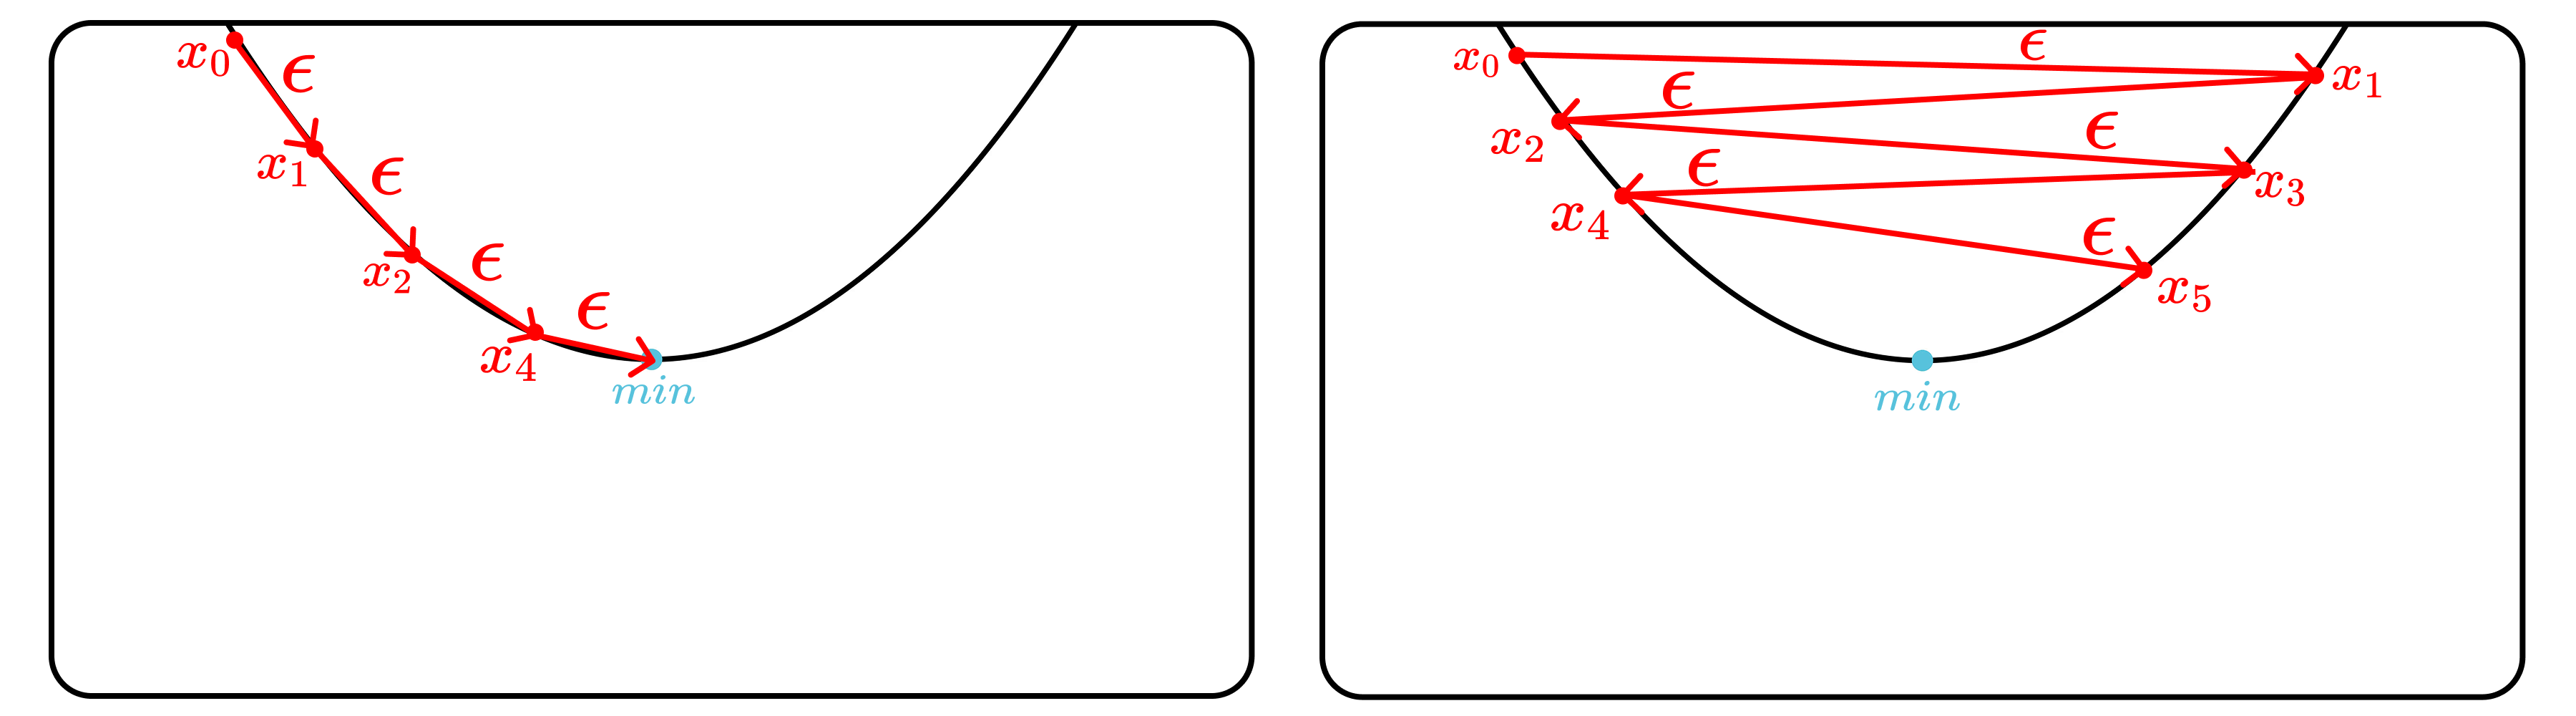
\includegraphics[width=1\linewidth]{../imagens/retropropagacao-gradiente/comparativo-de-passos.png}
    \caption{Comparativo do tamanho de passos em uma função polinomial.}
    \label{fig:comparativo-tamanho-do-passo}
\end{figure}

Na prática, escolher o valor da taxa de aprendizado é uma tarefa que irá depender de modelo em modelo, também irá variar com os diferentes métodos de otimização além da topologia da rede neural que está sendo construída. É sempre recomendado então experimentar diferentes tamanhos de passo, de forma que seja encontrado um que melhor se ajusta ao cenário que está sendo trabalhado.

Outro ponto que deve-se atentar é com relação as funções que estão sendo analisas ao utilizar o método do gradiente mas também qualquer otimizador que seja baseado nele. Se tivermos uma função convexa, em que seu formato lembra um funil, será bem mais fácil para o modelo encontrar o ponto de mínimo global daquela função. Mas se tivermos uma função não convexa, cheia de ondas e com muitos pontos de mínimos locais e pontos de sela, a convergência do modelo será pior, pois existe a chance de que ele fique preso em um ponto de mínimo local ou em um ponto de sela. Isso afeta diretamente o desempenho da rede neural que estará sendo criada, fazendo com que ela tenha métricas piores. O problema é que muitas das vezes a função $f(x)$ que estaremos interessados para calcular o desemepenho do modelo será não convexa, dificultando o seu aprendizado.

Na figura \ref{fig:funcao-convexa-nao-convexa} é possível ver o gráfico de duas funções diferentes, a primeira sendo uma função convexa e a segunda uma função não convexa.

\begin{figure}[h!]
\centering

% --- Gráfico 1: Função 3D Convexa ---
\begin{minipage}{0.48\textwidth}
    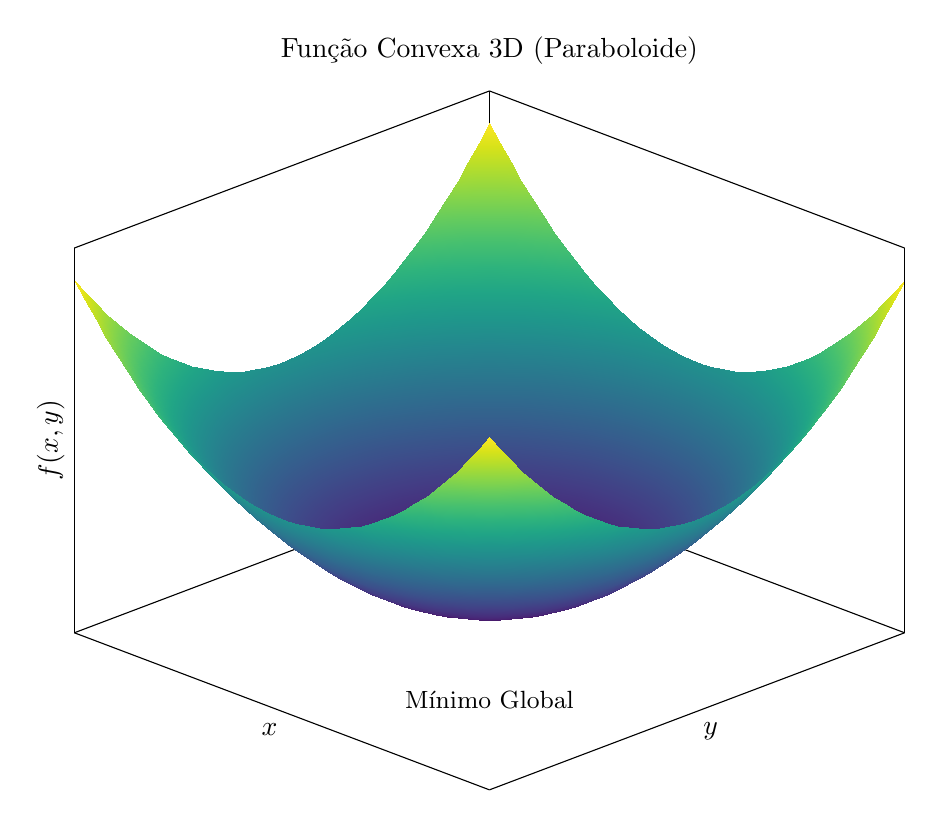
\begin{tikzpicture}
        \begin{axis}[
            title={Função Convexa 3D (Paraboloide)},
            xlabel=$x$,
            ylabel=$y$,
            zlabel={$f(x,y)$},
            xtick=\empty, ytick=\empty, ztick=\empty, % Remove marcações
            view={45}{30}, % Define o ângulo de visão 3D
            width=\textwidth,
            colormap/viridis, % Define o esquema de cores
        ]
        
        % Plot da superfície 3D z = x^2 + y^2
        \addplot3[
            surf, % Tipo de gráfico: superfície
            shader=interp, % Cores interpoladas para um visual suave
            domain=-2:2,
            domain y=-2:2,
            samples=40, % "Resolução" da malha
        ] {x^2 + y^2};
        
        % Marcador para o mínimo global
        \node at (axis cs:0,0,-2) [below, font=\small] {Mínimo Global};
        
        \end{axis}
        \label{fig:funcao-convexa}
    \end{tikzpicture}
\end{minipage}
\hfill % Espaço entre as figuras
% --- Gráfico 2: Função 3D Não-Convexa ---
\begin{minipage}{0.48\textwidth}
    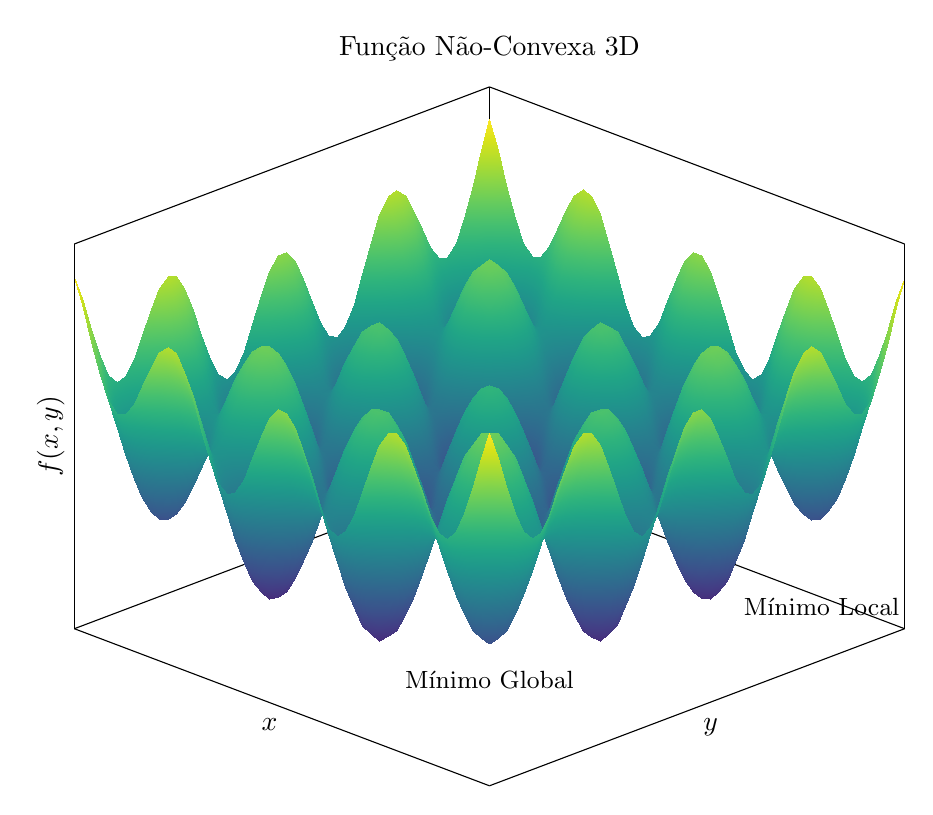
\begin{tikzpicture}
        \begin{axis}[
            title={Função Não-Convexa 3D},
            xlabel=$x$,
            ylabel=$y$,
            zlabel={$f(x,y)$},
            xtick=\empty, ytick=\empty, ztick=\empty,
            view={45}{30},
            width=\textwidth,
            colormap/viridis,
        ]
        
        % Plot da superfície com "ondinhas"
        % A função é um paraboloide + cossenos para criar as ondas
        \addplot3[
            surf,
            shader=interp,
            domain=-2.5:2.5,
            domain y=-2.5:2.5,
            samples=50,
        ] {(x^2+y^2)/5 + 2 - cos(deg(180*x)) - cos(deg(180*y))};
        
        % Marcadores para os mínimos
        \node at (axis cs:0,0,-1) [below, font=\small] {Mínimo Global};
        \node at (axis cs:2,2,0) [font=\small] {Mínimo Local};
        
        \end{axis}
        \label{fig-funcao-nao-convexa}
    \end{tikzpicture}
\end{minipage}
\caption{Comparação entre funções 3D convexas e não-convexas.}
\label{fig:funcao-convexa-nao-convexa}
\end{figure}

\subsection{Implementação em Python}

\begin{algorithm}[H]
\caption{O Método do Gradiente (Descida do Gradiente)}
\label{alg:gradient_descent}
\begin{algorithmic}[1]
\Require Taxa de aprendizado global $\epsilon$
\Require Parâmetros iniciais $\boldsymbol{\theta}$

\State Inicialize os parâmetros $\boldsymbol{\theta}$

\While{critério de parada não for atingido}
    \State Calcule o gradiente $\mathbf{g} \gets \nabla_{\boldsymbol{\theta}} L(\boldsymbol{\theta})$, usando \textbf{todo} o conjunto de treinamento
    \State Calcule a atualização: $\Delta \boldsymbol{\theta} \gets -\epsilon \mathbf{g}$
    \State Aplique a atualização: $\boldsymbol{\theta} \gets \boldsymbol{\theta} + \Delta \boldsymbol{\theta}$
\EndWhile
\end{algorithmic}
\end{algorithm}

Para implementar o método do gradiente utilizando Python e a biblioteca de cálculos Numpy, deve-se seguir como base a equação \ref{eq:metodo-do-gradiente}, criando uma classe implenta essa ferramenta, recebendo como parâmetros de entrada a taxa de aprendizado (\texttt{learning\_rate}), a função que se quer encontrar o ponto de mínimo (\texttt{function}), e um ponto inicial (\texttt{initial\_point}), que pode ser um conjunto de coordenadas aleatórias ou escolhidas pelo programador.

Outro ponto que deve ser destacado nas informações dessa função é de que ela também irá receber a derivada da função (\texttt{function\_prime}) que se quer descobrir o ponto de mínimo, pois não será feito cálculo simbólico para calcular o vetor gradiente. Dessa forma os cálculos serão mais rápidos. Além disso, também é preciso definir outros parâmetros auxiliares, como a quantidade máxima de iterações que o modelo irá seguir (\texttt{tolerance}), que são chamadas de épocas \texttt{epochs}, também será definida um grau de tolerância para o modelo, pois, podem existir casos em que a norma do vetor gradiente são será exatemente zero, mas um valor muito próximo de zero, assim a tolerância será responsável por definir qual valor dessa diferença será aceitável para o problema.

Por fim, um ponto interessante que é possível adicionar nessa função é uma lista, que irá armazenar todos os pontos que o modelo passou em cada uma de suas iterações, indicando o seu caminho pela função que está sendo estudada.

\begin{codelisting}{Classe completa do otimizador GradientDescent}{gd_class}
class GradientDescent:

    def __init__(self, function, function_prime, initial_point, learning_rate=0.001, epochs=100, tolerance=1e-6):
        self.f = function
        self.fp = function_prime
        self.ip = initial_point
        self.lr = learning_rate
        self.ep = epochs
        self.tol = tolerance
        self.path = []

    def update_step(self):
        for i in range(self.ep):
            self.path.append(self.ip)
            grad = self.fp(self.ip)
            if abs(grad) < self.tol: break
            self.ip = self.ip + self.lr * (-grad)
        return self.ip, self.path
\end{codelisting}

Note que a classe apresenta apenas dois métodos, o primeiro sendo o \texttt{\_\_init\_\_}, que inicializa os parâmetros da classe, e a \texttt{update\_step} a qual é responsável por implementar de fato o método do gradiente, ela irá retornar o ponto de mínimo e também a lista com os pontos pelos quais o modelo passou ao longo das iterações.

% ===================================================================
% A Retropropagação
% ===================================================================

\section{A Retropropagação: Aprendendo com os Erros}

Ainda no contexto de utilizar com o vetor gradiente para otimizar um modelo de rede neural, existe uma ferramenta que trabalha justamente com essse processo, ela é a retropropagação ou \textit{backpropagation} em inglês.

\begin{definicaomoderna}{\textbf{Definição:}}
A \textbf{retropropagação} é uma ferramenta que veio para permitir que redes que fazem o uso de unidades de neurônios possam aprender, para isso, o procedimento ajusta repetidamente os pesos das conexões da rede para minimizar a diferença entre o valor atual da saída do vetor da rede neural com o valor real desejado \parencite{BackpropagationArticle}.
\end{definicaomoderna}

Essa ferramenta foi introduzida para a comunidade científica pelos pesquisadores \textcite{BackpropagationArticle} no texto \textit{Learning Representations by Back-Propagating Errors}, e será explicada nesse capítulo de forma detalhada. Para issom \textcite{BackpropagationArticle} comecam introduzindo três diferentes funções que serão utilizadas ao longo do texto para deduzir o os conceitos da retropropagação do gradiente, sendo elas: a equação do neurônio, a função de ativação sigmoide e a função de custo do erro quadrático médio.

A primeira função, representada na equação xx, explica como um neurônio de uma camada densa irá funcionar quando recebe determinadas entradas.

\begin{equacaodestaque}{Equação do Neurônio}
    x_j = (\sum_i y_i \cdot w_{ji}) + b_j
    \label{eq:neuronio-camada-densa}
\end{equacaodestaque}

Sendo que:

\begin{itemize}
    \item $x_j$: representa a saída de um neurônio $j$;
    \item $y_i$: representa a entrada do neurônio $j$, a qual é resultado da saída de um neurônio $i$ da camada anterior;
    \item $w_{ij}$: representa o peso da conexão entre o neurônio $i$ com o neurônio $j$;
    \item $b_j$: representa o viés do neurônio $j$.
\end{itemize}

Caso você leitor decida olhar o artigo original, verá que os autores utilizaram notações diferentes na fórmula do neurônio, eles utilizam algo na forma $x_i = \sum_i y_i \cdot w_{ji}$, sem o viés, mas na prática, eles adicionam o viés como um peso extra que terá valor fixo igual a 1, na prática, ele pode ser tratado com um peso normal, por isso a notação mais simplificada \parencite{BackpropagationArticle}.

A segunda fórmula diz respeito a função de ativação que será utilizada, neste caso, \textcite{BackpropagationArticle} utilizam a sigmoide logísitca, representada na fórmula xx, mas eles explicam que essa função pode variar conforme o problema, porém recomendam ter uma derivada limitada além de ser não linear, para que o modelo possa aprender de forma mais efciente.

\begin{equacaodestaque}{Sigmoide Logística}
    y_j = \sigma(x_j) = \frac{1}{1 + e^{-x_j}}
    \label{eq:sigmoide}
\end{equacaodestaque}

Assim, a sigmoide é a função que irá transformar a saída do neurônio $x_j$ em uma saída $y_j$ que vai ser passada para o neurônio da camada seguinte. Além das duas notações da equação do neurônio, existe uma terceira, que já imbute a função de ativação na equação do neurônio, nesse livro, utilizaremos uma implementação de camadas, em que elas não possuem a função embutida, assim, caso decida que a saída da camada densa deva passar por uma função de ativação, ela deverá ser passada como uma camada separada, sendo algo da forma: camada densa, seguida de camada de ativação.

Por fim, a última equação que os autores discutem para entender a retropropagação é a da função de custo, ou também chamada de erro. No texto, \textcite{BackpropagationArticle} utilizam a função do erro quadrático médio (MSE), a qual calcula o erro entre a saída atual do modelo e o valor real desejado, depois ela eleva ao quadrado esse valor, e por último, divide por dois. Ela é dada pela equação:

\begin{equacaodestaque}{Erro Quadrático Médio (MSE)}
    E = \frac{1}{2} \sum_{c} \sum_{j} (y_{j, c} - d_{j, c})^2 
    \label{eq:mse}
\end{equacaodestaque}

Em que:

\begin{itemize}
    \item $E$: representa o valor do erro;
    \item $y_{j, c}$: representa o valor atual da saída do neurônio $j$ para o caso $c$;
    \item $d_{j, c}$: representa o valor desejado para o neurônio $j$ para o caso $c$
\end{itemize}

Considerando essas equações, \textcite{BackpropagationArticle} explicam que o objetivo é reduzir o valor do erro $E$, para isso, eles aplicam o método do gradiente para encontrar o ponto de mínimo da função MSE. Para isso, o primeiro passo é diferenciar o valor da função de erro em relação a cada um dos pesos da rede neural, assim, deve-se calcular $\partial E / \partial y_k$ para um caso específico $k$, e depois generalizar a situação. Assim, é possível encontrar uma expressão da forma:

\[
    \frac{\partial E}{\partial y_k} = \frac{\partial}{\partial y_k} \left[ \frac{1}{2} \sum_c \sum_k (y_{k, c} - d_{j, c})^2\right]
\]

O primeiro passo é suprimir a soma sobre os casos $c$, pois, consideramos apenas de um caso específico $k$, então a expressão se simplifica para:

\[
    \frac{\partial E}{\partial y_k} = \frac{\partial}{\partial y_k} \left[ \frac{1}{2} \sum_k (y_{k, c} - d_{j, c})^2\right]
\]

O próximo passo é abrir a soma, para isso, será considerado que existem $n$ neurônios na camada, assim, a expressão fica:

\[
    \frac{\partial E}{\partial y_k} = \frac{\partial}{\partial y_k} \left[ \frac{1}{2} \left( (y_1 - d_1)^2 + (y_2 - d_2)^2 + \cdots (y_k + d_k)^2 + \cdots + (y_n + d_n)^2 \right) \right]
\]

Note que todos os termos que não possuem o índice $k$, como a parte $(y_1 - d_1)^2$, serão valores constantes, e que estarão fora do obejtivo de calcular a derivada para o neurônio $k$, como eles são constantes, a sua derivada será igual a zero. Com base nisso, é possível obter uma versão ainda mais simplificada, sendo ela:

\[
    \frac{\partial E}{\partial y_k} = \frac{\partial}{\partial y_k} \left[ \frac{1}{2} (y_k + d_k)^2 \right]
\]

Agora, o último passo é aplicar a regra da cadeia na expressão que sobrou para poder calcular a derivada, neste caso, será considerado que $u = (y_k + d_k)$, assim a expressão final fica:

\[
    \frac{\partial E}{\partial y_k} = \frac{1}{2} \cdot 2u \cdot \frac{\partial u}{\partial y_k} = (y_k - d_k) \cdot 1 = (y_k - d_k)
\]

Voltando para o índice $j$ da notação inicial, é possível concluir que o gradiente do erro (para a função MSE) em relação a uma saída específica de um neurônio é dado pela diferença da saída da unidade pela resultado desejado, ou seja

\[
    \frac{\partial E}{\partial y_j} = (y_j - d_j) 
\]

O próximo passo proposto pelos autores, consiste em calcular o gradiente do erro em relação a entrada do neurônio $j$, para entender como o erro total muda em relação a uma variação na entrada do neurônio. Para isso, é preciso encontrar então a expressão $\partial E / \partial x_j$ \parencite{BackpropagationArticle}.

Assim, a primeira etepa é aplicar a regra da cadeia, pois, como a entrada do neurônio $x_j$ não aparece diretamente na equação do erro, é preciso aplicar a regra da cadeia, derivando o erro em relação a saída do neurônio $y_j$ e multiplicando esse resultado pela derivada da saída do neurônio em relação a sua entrada, assim, a expressão inicial é:

\[
    \frac{\partial E}{\partial x_j} = \frac{\partial E}{\partial y_j} \cdot \frac{\partial y_j}{\partial x_j}
\]

Perceba duas coisas nessa expressão, a primeira é que o primeiro termo é resultamente o primeiro que foi calculado e desenvolvido na expressão \ref{eq:gradiente-do-erro-em-relacao-a-saida-de-um-neuronio}, com isso, é possível substituir esse termo na expressão por $y_j - d_j$. A segunda informação, é de que o termo $\partial y_i / \partial x_j$ é justamente a derivada da função de ativação em relação a sua entrada, ou seja, $\sigma'(x_j)$, assim, a derivada da sigmoide será dada por:

\[
    \frac{d y_i}{d x_j} = y_j (1 - y_j)
\]

Sendo assim, a expressão final fica:

\[
    \frac{\partial E}{\partial x_j} = \frac{\partial E}{\partial y_j} \cdot y_j \cdot (1 - y_j)
\]

Note que é possível generalizar essa expressão, dessa forma o gradiente do erro da entrada de um neurônio é o gradiente do erro da saída do neurônio multiplicado pela derivada da função de ativação $\sigma'$ em relação a sua entrada $x_j$.

\begin{equacaodestaque}{Cálculo do Gradiente do Erro em Relação à Entrada de um Neurônio}
    \frac{\partial E}{\partial x_j} = \frac{\partial E}{\partial y_j} \cdot \sigma'(x_j)
    \label{eq:gradiente-do-erro-em-relacao-a-entrada-de-um-neuronio}
\end{equacaodestaque}

em que $\sigma'(x_j)$ representa a derivada de uma função de ativação qualquer, neste caso representa a sigmoide logística. Mas pode ser outra função, como a tangente hiperbólica ou a ReLU. Um ponto importante a ser destacado, é que como a retropropagação trabalha com o método do gradiente, as derivadas são parte essencial do algoritmo, utilizar funções de ativação que possuem derivadas complexas, ou que não podem ser derivadas em grande parte do seu domínio, acabam por difultar o algortimo. Caso a função possua uma derivada complexa, o cálculo do gradiente irá demorar mais, pois levará uma quantidade maior de operações para computar o valor da derivada.

O próximo passo vai mais além ainda, agora, como \textcite{BackpropagationArticle} explicam, o seu objetivo é entender como o gradiente muda em relação a um peso $w_ij$ específico da rede neural, para isso, é preciso calcular a expressão $\partial E / \partial w_{ij}$, note mais uma vez que o peso $w_{ij}$ não aparece diretamente na equação do erro, assim, é necessário mais uma vez aplicar a regra da cadeia para calcular essa derivada. Assim, a expressão inicial é:

\[
    \frac{\partial E}{\partial w_{ij}} = \frac{\partial E}{\partial x_j} \cdot \frac{\partial x_j}{\partial w_{ij}}
\]

Note que o primeiro termo da expressão é justamente o que foi calculado na equação \ref{eq:gradiente-do-erro-em-relacao-a-entrada-de-um-neuronio}, assim, é preciso calcular apenas o segundo termo, $\partial x_i / \partial w_{ij}$, ou seja, a derivada do neurônio em relação a um peso específico. Assim, tem-se a expressão incial:

\[
    \frac{\partial x_j}{\partial w_{ij}} = \frac{\partial}{\partial w_{ij}} \left[ \left( \sum_i y_i \cdot w_{ji} \right) + b_j\right]
\]

Note que o viés, dado por $b_j$ é uma constante, e por isso, não depende do peso $w_{ij}$, então a sua derivada será igual a zero, isso nos permite simplicar a expressão para:

\[
    \frac{\partial x_j}{\partial w_{ij}} = \frac{\partial}{\partial w_{ij}} \left[\sum_i y_i \cdot w_{ji}\right]
\]

Em seguida, é possível abrir a soma, assim, temos a expressão:

\[
    \frac{\partial x_j}{\partial w_{ij}} = \frac{\partial}{\partial w_{ij}} \left[ (y_1 \cdot w_{j1}) + (y_2 \cdot w_{j2}) + \cdots (y_i \cdot w_{ji}) + \cdots (y_n \cdot w_{jn})\right]
\]

Note que para qualquer termo que o índice não é $w_{ji}$ a derivada será iguala zero, pois eles serão constantes em relação ao peso $w_{ji}$, dessa forma, é possível simplificar mais uma vez a expressão obtendo:


\[
    \frac{\partial x_j}{\partial w_{ij}} = \frac{\partial}{\partial w_{ij}} \left[  y_i \cdot w_{ji} \right]
\]

Como $y_i$ é uma constante em relação a $w_ij$ a derivada final será dada por:

\[
    \frac{\partial x_j}{partial w_{ij}} = y_i
\]

Agora é possível voltar para a expressão inicial, obtendo então a expressão final para o gradiente do erro em relação a um peso específico da rede neural, sendo ela:

\begin{equacaodestaque}{Cálculo do Gradiente do Erro em Relação a um Peso de um Neurônio}
    \frac{\partial E}{\partial w_{ij}} = \frac{\partial E}{\partial x_j} \cdot y_i = \frac{\partial E}{\partial y_j} \cdot \sigma'(x_j) \cdot y_i
    \label{eq:gradiente-do-erro-em-relacao-a-um-peso-de-um-neuronio}
\end{equacaodestaque}

Assim, é possível concluir que o gradiente do erro em relação a um peso específico de um neurônio é dado pelo gradiente do erro da saída do neurônio multiplicado pela derivada da função de ativação em relação a sua entrada e, por fim, multiplicado pela entrada do neurônio.

O próximo passo não está no artigo original, ele envolve entender como o erro varia em relação a um viés de um neurônio específico, ou seja, é preciso calcular a expressão $\partial E / \partial b_j$. Note que mais uma vez o viés $b_j$ não aparece diretamente na equação do erro, ele está dentro da equação do neurônio, assim, novamente é preciso aplicar a regra da cadeia para encontrar essa derivada, assim, a expressão inicial é dada por:

\[
    \frac{\partial E}{\partial b_j} = \frac{\partial E}{\partial x_j} \cdot \frac{\partial x_j}{\partial b_j}
\]

A primeira expressão, $\partial E / \partial x_j$, já foi calculada na equação \ref{eq:gradiente-do-erro-em-relacao-a-entrada-de-um-neuronio}, assim, é preciso focar apenas na segunda parte da expressão, $\partial x_j / \partial b_j$, que avalia como a saída do neurônio $x_j$ varia em relação ao viés $b_j$. Com base, nisso, é possível chegar na expressão:

\[
    \frac{\partial E}{\partial b_j} = \frac{\partial}{\partial b_j} \left[ \left( \sum_k y_k \cdot w{jk} \right) + b_j \right]
\]

Note que os termos que não possuem o viés, como a parte que faz a soma da multiplicação das entradas pelos pesos, $\sum_l y_k \cdot w_{jk}$, são constantes em relação ao viés, portanto, a sua derivada será igual a zero, de tal forma que é possível simplificar a expressão para:

\[
        \frac{\partial E}{\partial b_j} = \frac{\partial}{\partial b_j} \left[ b_j \right]
\]

Com base nessa expressão, é possível concluir que a derivada da saída do neurônio em relação ao viés é igual a 1. Assim, voltando para a expressão inicial, temos que o gradiente do erro em relação ao viés de um neurônio específico é dado pelo gradiente do erro da entrada entrada total desse neurônio, ou seja:

\begin{equacaodestaque}{Cálculo do Gradiente do Erro em Relação a um Viés de um Neurônio}
    \frac{\partial E}{\partial b_j} = \frac{\partial E}{\partial x_j} \cdot 1 = \frac{\partial E}{\partial y_j} \cdot \sigma'(x_j)
    \label{eq:gradiente-do-erro-em-relacao-a-um-vies-de-um-neuronio}
\end{equacaodestaque}

\subsection{Utilizando o Gradiente Descendente para Atualizar os Pesos e Vieses}

Já que é possível calcular o gradiente do erro em relação a um peso específico de um neurônio, e também em relação a um viés específico de um neurônio, o próximo passo proposto pelos autores é utilizar o método do gradiente como uma forma de atualizar os pesos (e também os vieses no nosso caso) da rede neural, de forma a minimizar o valor do erro com pequenas atualizações em cada um desses parâmetros \parencite{BackpropagationArticle}.

Note que o método do gradiente, explicado na seção anterior diz que para atualizar um parâmetros, é preciso pegar o valor atual do parâmetro, e subtrair dele o valor do gradiente multiplicado pelo tamanho do passo (ou taxa de aprendizado). dessa forma, a regra de atualização para um peso específico é dada pela equação \ref{eq:regra-de-atualizacao-de-um-peso-atraves-do-metodo-do-gradiente}


\begin{equacaodestaque}{Regra de Atualização de um Peso Através do Método do Gradiente}
    w_{t+1} = w_{t} - \epsilon \frac{\partial E}{\partial w}
    \label{eq:regra-de-atualizacao-de-um-peso-atraves-do-metodo-do-gradiente}
\end{equacaodestaque}

Em que:

\begin{itemize}
    \item $w_{t+1}$ representa o valor do peso atualizado após o incremento do método do gradiente;
    \item $w_t$ representa o valor inicial do peso na iteração $t$;
    \item $\epsilon$ representa o tamanho do passo / taxa de aprendizado;
    \item $\partial E / \partial w$ representa o gradiente do erro em relação ao peso.
\end{itemize}

Analogamente, a regra de atualização de um viés pelo método do gradiente é dada pela equação \ref{eq:regra-de-atualizacao-de-um-vies-atraves-do-metodo-do-gradiente}

\begin{equacaodestaque}{Regra de Atualização de um Viés Através do Método do Gradiente}
    b_{j, t+1} = b_{j, t} - \epsilon \frac{\partial E}{\partial b_j}
    \label{eq:regra-de-atualizacao-de-um-vies-atraves-do-metodo-do-gradiente}
\end{equacaodestaque}

Neste caso, $b_{j, t+1}$ representa o valor final de um viés $j$ após o incremento do método e $b_{j, t}$ o valor inicial do viés $j$.

Um ponto a ser destacado, é que quando estiver trabalhando com uma camada densa de neurônios, você não irá lidar com um neurônio específico, e sim como uma conjunto inteiro deles. Dessa forma, eles estrão distribuidos de forma vetorizada, que que terá um vetor de viéses, uma matriz de pesos e um vetor de neurônios. Assim, as expressões {eq:regra-de-atualizacao-do-vetor-de-pesos-atraves-do-metodo-do-gradiente} e \ref{eq:regra-de-atualizacao-do-vetor-de-vieses-atraves-do-metodo-do-gradiente}, resumem as regras de atualização de pesos e vieses, respectivamente, para casos em que estiver lidando com um conjunto de vetores ao invés de somente um dado.

\begin{equacaodestaque}{Regra de Atualização do Vetor de Pesos Através do Método do Gradiente}
    \mathbf{w}_{t+1} = \mathbf{w}_t - \epsilon \nabla_{\mathbf{w}} E
    \label{eq:regra-de-atualizacao-do-vetor-de-pesos-atraves-do-metodo-do-gradiente}
\end{equacaodestaque}

\begin{equacaodestaque}{Regra de Atualização do Vetor de Vieses Através do Método do Gradiente}
    \mathbf{b}_{t+1} = \mathbf{b}_t - \epsilon \nabla_{\mathbf{b}} E
    \label{eq:regra-de-atualizacao-do-vetor-de-vieses-atraves-do-metodo-do-gradiente}
\end{equacaodestaque}

\subsection{Entendendo Como o Gradiente É Propagado ao Longo de Muitas Camadas}

Por fim, com base no que foi explicado até agora, é possível entender melhor como o gradiente passa de uma acamada para a outra durante a retropropagação, para isso será analisada um rede com quatro camadas densas, sendo elas:

\begin{itemize}
    \item \textbf{Camada 1 (Entrada):}: Ela possui neurônios com o indice $i$;
    \item \textbf{Camada 2 (Oculta 1):}: Ela possui neurônios com o indice $j$;
    \item \textbf{Camada 3 (Oculta 3):}: Ela possui neurônios com o indice $k$;
    \item \textbf{Camada 4 (Oculta 3):}: Ela possui neurônios com o indice $l$;
\end{itemize}

O objetivo é calcular o gradiente de um peso da primeira camada de pesos, $w_{ji}$, ou seja, é um peso que conecta um neurônio da camada $i$ com um neurônio da camada $j$. Assim, o primeiro passo é utilizar a fórmula \ref{eq:gradiente-do-erro-em-relacao-a-um-peso-de-um-neuronio}, que calcula o gradiente do erro em relação a um peso quaquer.

\[
    \frac{\partial E}{\partial w_{ij}} = \frac{\partial E}{\partial x_j} \cdot y_i
\]

Para encontrar esse gradiente, é preciso desenvolver a expressão $\partial E / \partial x_j$, que representa o gradiente do erro da entrada de um neurônio $j$ da primeira camada oculta. Para isso, é possível utilizar como base a equação \ref{eq:gradiente-do-erro-em-relacao-a-entrada-de-um-neuronio}, obtendo então:

\[
    \frac{\partial E}{\partial x_j} = \frac{\partial E}{\partial y_j} \cdot \sigma'(x_j)
\]

Nessa expressão, $\sigma'(x_j)$ representa a função de ativação, já o termo $\partial E / \partial y_j$ representa o gradiente que está vindo ca camada de cima, o qual é dado por:

\[
    \frac{\partial E}{\partial x_j} = \sum_k \frac{\partial E}{\partial x_k} \cdot w_{kj}
\]

Juntando os dois termos:

\[
    \frac{\partial E}{\partial x_j} = \left( \sum_k \frac{\partial E}{\partial x_k} \cdot w_{kj} \right) \sigma'(x_j)
\]

Agora, é preciso calcular o termo $\partial E / \partial x_j$, de forma que será possível trazer o gradiente da camada de saída $l$, assim temos:

\[
    \frac{\partial E}{\partial x_k} = \left( \sum_k \frac{\partial E}{\partial x_l} \cdot w_{lk} \right) \cdot \sigma'(x_k)
\]

Em que $\partial E / \partial x_l$ representa o primeiro gradiente, ele é calculado na camada de saída.

Por último, é preciso combinar essas expressões, encontrando como resultado a expressão:

\[
    \frac{\partial E}{\partial w_{ij}} = \left( \sum_k \left[ \left( \sum_l \frac{\partial E}{\partial x_l} \cdot w_{lk} \right) \sigma'(x_k) \right] \cdot w_{kj} \right) \sigma(x_j) \cdot y_i
\]

Com base nessa expressão, é possível concluir que o gradiente de uma camada inicial é proporcional a uma cadeia de multiplicações dos pesos e das derivadas das funções de ativação das camadas posteriores, de forma que é possível simplificar isso para:

\[
    \frac{\partial E}{\partial w_{\text{primeira camada}}} \propto (\text{gradiente da saída}) \cdot (w_{\text{camada 3}} \cdot \sigma'_{\text{camada 3}}) \cdot (w_{\text{camada 2}} \cdot \sigma'_{\text{camada 2}})
\]

Generalizando essa expressão, é possível concluir que o gradiente para uma camada é dado ela equação \ref{eq:gradiente-para-n-camadas}.

\begin{equacaodestaque}{Gradiente para N Camadas}
    \delta^{(L)} = \left( \left( \textbf{W}^{(L+1)} \right)^T \delta^{(L+1)} \right)  \odot \sigma'(x^{(L)})
    \label{eq:gradiente-para-n-camadas}
\end{equacaodestaque}

Em que: 

\begin{itemize}
    \item $L$: Representa o índice de uma camada, podendo ser um valor entre $1$ (indicando que é uma camada de entrada) ou $n$ (indicando que é uma camada de saída);
    \item $\textbf{W}^{(L)}$: Representa a matriz dde pesos que conecta a camada $L - 1$ à camada $L$;
    \item $b^{(L)}$: Representa o vetor de viés da camada $L$;
    \item $x^{(L)}$: Representa o vetor de entradas totais para os neurônios da camada $L$ antes da ativação;
    \item $y^{(L)}$: Representa o vetor de saídas da camada $L$
    \item $\delta^{(L)}$: Representa o vetor do gradienye na camada $L$;
    \item $\sigma'(x^{(L)})$: Representa o vetor contendo a derivada da função de ativação para cada neurônio da camada $L$;
    \item $\odot$: O produto de Hadamard, que significa multiplicação elemento a elemento.
\end{itemize}

Assim, é possível entender como o gradiente irá se propagar ao longo de uma rede neural. Esse ponto é um dos mais importantes, pois é possível considerar que ele terá uma grande relação com as funções de ativação que são utilizadas. Essa é uma relação complicada, pois, enquanto um determinado tipo de função possa causar um tipo de problema no cálculo do gradiente, e por isso não deve ser uma opção viável para ser escolhida para resolver um problema, optar por outra família de função também pode acarretar outro tipo de problema com o gradiente.

Para isso, o capítulo \ref{cap:ativacao-sigmoidais} foca em entender as pricipais funções sigmoidais, como a sigmoide e a tangente hiperbólica, e como essas possuem uma forte relação com o problema do desaparecimento de gradientes. Em seguida, o capítulo \ref{cap:ativacao-retificadoras} busca introduzir as funções retificadoras, como a ReLU, e como elas podem ser uma alternativa para contornar esse problema. Contudo, isso não as torna perfeitas, elas ainda são suceptíveis à outro tipo de problema: a explosão de gradientes; e, no caso da ReLU: o problema dos neurônios agonizantes.

% ===================================================================
% Otimizadores Baseados em Gradiente
% ===================================================================

\section{Otimizadores Baseados em Gradiente: Melhorando o Gradiente Descendente}

Como \textcite{BackpropagationArticle} explicam logo ao terminar a dedução do cálculo da atualização dos pesos utilizando o método do gradiente, esse processo pode ser bastante lento quando comparado com métodos que fazem uso de derivadas de segunda ordem, que certamente são mais caras para serem implementadas no computador. Assim, os autores recomendam uma variação do método do gradiente que faz uso de momentum com intuito de acelerar a convergência a um custo computacional menor que o de implementar derivadas de segunda ordem \parencite{BackpropagationArticle}.

\subsection{Método do Gradiente com Momentum}

Uma boa analogia para entender como o método do gradiente com momentum funciona é pensar é uma pedra rolando morro abaixo. No começo, quando ela não havia pegado muita velocidade, ela demorava para rolar e dependendo podia quase parar em algum pedaço do morro, mas conforme foi descendo, foi ganahando mais velocidade, de forma que quando chegar no final do morro, a sua velocidade será bem maior do que quando estava no topo do mesmo. Essa variante funciona de forma parecida a esse cenário.

Da mesma forma que o método do gradiente não surgiu originalmente no contexto do aprendizado de máquina, a sua variante com momentum não foi diferente. Um os artigos que trabalha com esse conceito de utilizar o momentum para acelerar a velocidade do método do gradiente e com isso obter uma convergência mais rápida é o \textit{Some methods of speeding up the convergence of iteration methods}, do pesquisador \textcite{polyak1964}, nele o autor busca criar métodos iterativos mais rápidos para resolver equações funcionais. Para isso, ele introduz um método de "dois passos", que consiste na junção do método do gradiente com um segundo termo que dá inércia ao método, por último, ele justifica que esse método trás de fato uma convergência mais veloz quando comparado com métodos como o do gradiente.

Contudo, assim como a grande maioria dos conceitos matemáticos, essa ideia demorou a ser implementada para o aprendizado de máquina, e com o surgimento da retropropagação, como demonstrado por \parencite{BackpropagationArticle}, em seu artigo, o método do gradiente com momentum se tornou uma excelente opção para garantir uma convergência mais rápida. Esse método é representado pela equação \ref{eq:metodo-do-gradiente-com-momentum-de-polyak}

\begin{equacaodestaque}{Método do Gradiente com Momentum de Polyak}
        x_{n+1} = x_n - \epsilon \nabla f(x_n) + \beta(x_n - x_{n-1})
    \label{eq:metodo-do-gradiente-com-momentum-de-polyak}
\end{equacaodestaque}

Em que:

\begin{itemize}
    \item $x_{n+1}$: Representa as coordenadas do ponto após a iteração do método;
    \item $x_n$: Representa as coordenadas do ponto na iteração $n$;
    \item $\epsilon$: Representa a taxa de aprendizado / tamanho do passo
    \item $\beta$: Representa a "inércia", controlando a influência do passo anterior no passo atual;
    \item $x_{n-1}$: Representa as coordenadas do ponto na iteração anterior.
\end{itemize}

Para calcular $\beta$, \textcite{polyak1964} determina que será utilizada a expressão:

\[
    \beta = \left( \frac{\sqrt{M} - \sqrt{m}}{\sqrt{M} + \sqrt{m}} \right)^2
\]

Em que $M$ representa o maior valor da matriz hessiana $m$ é o menor valor no ponto de mínimo da função. Isso significa que esses valores não são conhecidos de antemão. Contudo o maior problema da fórmula proposta por Polyak é que ela exige muitos cálculos, imagine ter que calcular a matriz hessiana de uma função de perda para uma rede que possui milhares ou até milhões de parâmetros, isso é muita coisa e também muito demorado. Assim, no artigo da retropropagação, \textcite{BackpropagationArticle}, apresentam uma fórmula diferente, com intuito dimunuir a quantidade de cálculos a serem feitas, mas mantendo a principal caracterísitca do método do gradiente com momentum: a inércia; ela é dada pela equação \ref{eq:metodo-do-gradiente-com-momentum-da-retropropagacao}

\begin{equacaodestaque}{Método do Gradiente com Momentum Usado na Retropropagação}
        \Delta w (t) = \epsilon \nabla f(x) + \alpha \Delta w(t-1)
    \label{eq:metodo-do-gradiente-com-momentum-da-retropropagacao}
\end{equacaodestaque}

Em que:

\begin{itemize}
    \item $\Delta w(t)$: Representa a variação nos pesos;
    \item $\epsilon$: Representa a taxa de aprendizado;
    \item $\nabla f(x)$: Representa o gradiente;
    \item $\alpha$: Representa um fator de decaimento exponencial entre 0 e 1 que determina a contribuição do gradiente passado para o gradiente futuro.
\end{itemize}

\subsubsection{Implementação em Python}

\begin{algorithm}[H]
\caption{O Método do Gradiente com Momentum (versão de Rumelhart et al.)}
\label{alg:momentum_rumelhart}
\begin{algorithmic}[1]
\Require Taxa de aprendizado global $\epsilon$
\Require Coeficiente de momentum $\alpha$
\Require Parâmetros iniciais $\boldsymbol{\theta}$

\State Inicialize a atualização anterior: $\Delta\boldsymbol{\theta} \gets \mathbf{0}$
\State Inicialize os parâmetros $\boldsymbol{\theta}$

\While{critério de parada não for atingido}
    \State Calcule o gradiente $\mathbf{g} \gets \nabla_{\boldsymbol{\theta}} L(\boldsymbol{\theta})$
    \State Calcule a atualização atual: $\Delta\boldsymbol{\theta} \gets -\epsilon \mathbf{g} + \alpha \Delta\boldsymbol{\theta}$
    \State Aplique a atualização: $\boldsymbol{\theta} \gets \boldsymbol{\theta} + \Delta\boldsymbol{\theta}$
\EndWhile
\end{algorithmic}
\end{algorithm}

\subsection{Método do Gradiente em Mini-Batch}

\subsection{Método do Gradiente Estocástico}

\begin{equacaodestaque}{Método do Gradiente Estocástico}
        \theta_{\text{novo}} = \theta_{\text{antigo}} - n \nabla J(\theta; x^{(i); y^{(i)}}
    \label{eq:metodo-do-gradiente-com-momentum-da-retropropagacao}
\end{equacaodestaque}

\subsubsection{Implementação em Python}

\subsection{Gradiente Acelerado de Nesterov}

\begin{equacaodestaque}{Gradiente Acelerado de Nesterov}
    \begin{aligned}
        y_k     &= x_k + \beta(x_k - x_{k-1})   && \text{1. Calcula uma predição futura (lookahead) } y_k, \\
                &                               && \text{   dando um passo na direção do momento anterior.} \\[1em]
        x_{k+1} &= y_k - \epsilon \nabla f(y_k) && \text{2. Calcula o gradiente em } y_k \text{ (na predição)} \\
                &                               && \text{   e atualiza os pesos } x_k \text{ a partir de } y_k.
    \end{aligned}
    \label{eq:gradiente-acelerado-de-nesterov}
\end{equacaodestaque}

Em que:

\begin{itemize}
    \item $y_k$: Representa o ponto de "lookahead";
    \item $x_k$: Representa os parâmetros na iteração $k$;
    \item $x_{k-1}$: Representa os parâmetros na iteração $k-1$;
    \item $\beta$: Representa
    \item $x_{k+1}$: Representa os parâmetros na iteração $k+1$;
    \item $epislon$: Representa a taxa de aprendizado;
    \item $\nabla f(y_k)$: Representa o vetor gradiente calculado no ponto de "lookahead"
\end{itemize}

\subsubsection{Implementação em Python}

\section{Otimizadores Modernos Baseados em Gradiente: A Era das Taxas de Apredendizado Adaptativas}

Conforme os anos foram passando, foram surgindo novos algoritmos de otimização baseados na ideia da descida do gradiente. A partir dos anos 2010, otimizadores como o AdaGrad foram ganhando popularidade na comunidade, principalmente por apresentar uma diferença notavável quando comparados com os algoritmos clássicos: a utilização de diferentes parâmetros de representado a taxa de aprendizado, de forma que ela pudesse ser adptável para cada um dos conjuntos de características que estavam sendo analisadas.

Essa seção busca justamente explorar esses otimizadores, explicando suas fórmulas e algortítmos, suas vantagens quando comparados com os métodos tradicionais. Além disso, é possível ver uma evolução graduau em como cada algoritmo sucessor busca complementar pequenos erros os métodos anteriores possuíam.

\subsection{Adadptive Gradient Algorithm (AdaGrad)}

Apresentado para a comunidade científica no texto \textit{Adaptive Subgradient Methods for Online Learning and Stochastic Optimization}, o Adadptive Gradient Algorithm (AdaGrad), \textcite{AdaGradMethod} o descrevem metafóricamente como uma adpatação dos métodos iterativos baseados em gradiente, que nos permite encontrar agulhas em palheiros em forma de características muito preditivas, mas raramente vistas.

O que os autores se referem ao ato de "encontrar agulhas em palheiros", está ligado diretamente na forma como o AdaGrad atua para melhorar o desempenho de um modelo tanto para reconhecer caracteríticas que são muito frequentes nos dados de treino quando características que são mais raras. Como \textcite{AdaGradMethod} explicam, esse método faz uso de múltiplas taxas de aprendizado, assim caracterítiscas muito frequentes recebem uma taxa de aprendizado pequena, enquanto caraterísticas menos frequentes recebem uma taxa de aprendizado maior.

Dessa forma, o modelo que está sendo treinado conseque garantir melhores métricas durante o seu aprendizado, pois estará aprendendo sobre aquilo que aparece muito nos dados de treino, mas, quando aparecer algo diferente e menos comum, ele irá "prestar mais atenção" devido à maior taxa de aprendizado nessas características.

O AdaGrad veio como uma forma de aplicar técnicas de aprendizado-teórico para problemas online e aprendizado estocástico, focando concretamente no métodos de (sub)gradiente, de forma que a representação desse algoritmo pode ser vista no bloco de algoritmo \ref{alg:adagrad}.

\begin{algorithm}[H]
    \caption{AdaGrad}
    \label{alg:adagrad}
    \begin{algorithmic}[1]

    \State \textbf{ENTRADA:} $\eta > 0, \delta \ge 0$
    \State \textbf{VARIÁVEIS:} $s \in \mathbb{R}^d, H \in \mathbb{R}^{d \times d}, g_{1:t,i} \in \mathbb{R}^t$ para $i \in \{1,\dots,d\}$
    \State \textbf{INICIALIZE:} $x_1 = 0, g_{1:0} = []$

    \For{$t = 1$ até $T$}
        \State Incorre na perda $f_t(x_t)$
        \State Recebe o subgradiente $g_t \in \partial f_t(x_t)$ de $f_t$ em $x_t$
        \State \textbf{ATUALIZE} $g_{1:t} = [g_{1:t-1} g_t], \quad s_{t,i} = \|g_{1:t,i}\|_2$
        \State \textbf{DEFINA} $H_t = \delta I + \text{diag}(s_t), \quad \Psi_t(x) = \frac{1}{2}\langle x, H_t x \rangle$
    \EndFor

    \State
    \State \textbf{Atualização de Subgradiente Primal-Dual (3):}
    \State $x_{t+1} = \underset{x \in X}{\text{argmin}} \left\{ \eta \left\langle \frac{1}{t} \sum_{\tau=1}^t g_\tau, x \right\rangle + \eta \phi(x) + \frac{1}{t} \Psi_t(x) \right\}$

    \State
    \State \textbf{Atualização Composta de Mirror Descent (4):}
    \State $x_{t+1} = \underset{x \in X}{\text{argmin}} \left\{ \eta \langle g_t, x \rangle + \eta \phi(x) + B_{\Psi_t}(x, x_t) \right\}$

    \end{algorithmic}
\end{algorithm}

Note que essa definição foge do contexto de aprendizado de máquina, de forma que ela pode ser simplificada em várias partes a fim de criar uma fórmula mais resumida. No algoritmo, a linha $s_{t_,i} = [g_{1:t,i}]_2$ calcula a norma L2, ou seja, o comprimento do vetor, de todos os gradientes passados para um único parâmetro i. Dessa forma, a matriz $H_t$ armazena esses valores em sua diagonal. Quando está sendo calculada a norma L2 ao quadrado, como neste caso, é o mesmo que somar os quadrados de cada componente, assim, sua representação pode ser simplificada para $G_t = G_{t-1} + g_t \odot g_t$, que é uma maneira simplificada de calcular a soma dos quadrados dos gradientes passados. Neste caso, o termo $G_t$ é uma adpatação da matriz $H_t$, só que ao invés de simbolizar uma matriz que armazena a norma dos gradientes, isso é feito por em forma de um vetor.

Ainda é possível fazer uma segunda simplificação no algoritmo, agora na linha que calcula $x_{t+1} = armmin{}$, pois o que essa linha representa é uma forma matemática de descrever "encontre o próximo ponto $x_{t+1}$ que minimiza uma combinação d gradiente e da distância em relação ao ponto atual". Como em redes neurais, não existem restrições tão complexas, a solução para esse problema se resume a dar um passo na direção do gradiente, com o tamanho do passo dividio pelo acumulador de gradientes.

Após essas duas simplificações para o cenário de aprendizado de máquina, é possível chegar em uma fórmula semelhante a equação \ref{eq:adagrad-simplificado}

\begin{equacaodestaque}{Adadptive Gradient Algorithm (AdaGrad) Simplificado para Redes Neurais}
    \begin{aligned}
        G_t          &= G_{t-1} + g_t \odot g_t && \text{1. Acumula a soma dos quadrados dos gradientes }(g_t) \\
                     &                           && \text{   na matriz } G_t \text{ a cada passo.} \\[1em]
        \theta_{t+1} &= \theta_t - \frac{n}{\sqrt{G_t + \epsilon}} \odot g_t && \text{2. Atualiza os parâmetros }(\theta). \text{ A taxa de aprendizado } (n) \\
                     &                           && \text{   é adaptada para cada parâmetro, sendo dividida} \\
                     &                           && \text{   pela raiz da soma acumulada } G_t.
    \end{aligned}
    \label{eq:adagrad-simplificado}
\end{equacaodestaque}

Em que:

\begin{itemize}
    \item $G_t$: Representa o vetor da soma dos quadrados dos gradientes na iteração $t$;
    \item $G_{t-1}$: Representa o vetor da soma dos quadrados dos gradientes na iteração $t-1$;
    \item $g_t$: Representa o vetor gradiente calculado na iteração $t$;
    \item $\theta_{t+1}$: Representa o vetor de parâmetros na iteração $t+1$;
    \item $\theta_t$: Representa o vetor de parâmetros na iteração $t$;
    \item $n$: Representa a taxa de aprendizado adpatada para cada parâmetro;
    \item $\epsilon$: Representa a taxa de aprendizado geral;
    \item $\odot$: Representa o produto de Hadamard.
\end{itemize}


\subsubsection{Implementação em Python}

\subsection{RMSProp}

\begin{equacaodestaque}{RMSProp}
    \begin{aligned}
        E[g^2]_t     &= \gamma E[g^2]_{t-1} + (1 - \gamma)(g_t \odot g_t) && \text{1. Calcula a média móvel dos quadrados dos} \\
                     &                                                   && \text{   gradientes. O fator } \gamma \text{ (decaimento) dá mais} \\
                     &                                                   && \text{   peso aos gradientes mais recentes.} \\[1em]
        \theta_{t+1} &= \theta_t - \frac{n}{\sqrt{E[g^2]_t + \epsilon}} \odot g_t && \text{2. Atualiza os parâmetros. A taxa de aprendizado é} \\
                     &                                                            && \text{   dividida pela raiz da média móvel, evitando que} \\
                     &                                                            && \text{   a atualização se torne pequena demais com o tempo.}
    \end{aligned}
    \label{eq:RMSProp}
\end{equacaodestaque}

\subsubsection{Implementação em Python}

\subsection{Adaptive Moment Estimation (Adam)}

Uma evolução natural dos algortitmos de otimização AdaGrad e RMSProp é o Adam ou Adaptive Moment Estimation. Esse algortimo foi apresentado pelos pesquisadores \textcite{AdamMethod}, no artigo \textit{Adam: A Method for Stochastic Optimization}, ele veio para ser um método de otimização estocástica que requere apenas gradientes de primeira ordem com poucos requisitos de memória.

Para isso, o Adam computa taxas de aprendizado individuais para diferentes parâmetros para estimações do priemiro e segundo momento do gradiente, de forma que ele é capaz de combinar as vantagens do AdaGrad, que trabalha bem com gradientes esparsos, e o RMSProp, que trabalha bem on-line e em configurações não-estacionárias \parencite{AdamMethod}.

O Adam recebe como entradas uma taxa de aprendizado ($\alpha$), decebe dois valores $\beta_1$ e $\beta_2$ que representam as taxas de decaimento esponencial para as estimativas de momento em um conjunto de intervalos $[0, 1)$. Além disso, assim como todo método de otimização ele também recebe em sua entrada uma função de perda $f(\theta)$ bem como os parâmetros iniciais $\theta_0$.

O primeiro passo do método consiste em inicializar os vetores de primeiro ($m_0$) e segundo ($v_0$) momento bem como o passo do tempo $t$, para isso, ele coloca como zero os seus valores iniciais. Em seguida, é iniciado o loop de iterações do método, que só irá parar quando $\theta_t$ convergir. Nesse loop, primeiramente é feito um incremento no valor do passo de tempo, depois é calculado o valor do gradiente no tempo $t$, o qual é armazenado em $g_t$. Com base nessa nova variável é atualizado uma estimativa enviesada no primeiro momento, armazenada em $m_t$, em seguida, é feita uma segunda estimativa também enviesada só que agora no segundo momento. Essas estimativas são então corridas pelo método que com base nelas é feito a atualização dos parâmetros e assim uma iteração termina. Caso o método convirja ele irá retornar como resultado os parâmetros $\theta_t$.

Esse método pode ser visto no bloco de algoritmo \ref{alg:adam}.

\begin{algorithm}[H] % A opção [H] tenta colocar o algoritmo exatamente aqui
    \caption{Adam, nosso algoritmo proposto para otimização estocástica}
    \label{alg:adam}
    \begin{algorithmic}[1] % O [1] habilita a numeração das linhas

    \Require Taxa de aprendizado $\alpha$
    \Require Taxas de decaimento exponencial para as estimativas de momento $\beta_1, \beta_2 \in [0, 1)$
    \Require Função objetivo estocástica com parâmetros $\theta$, $f(\theta)$
    \Require Vetor de parâmetros inicial $\theta_0$

    \State $m_0 \leftarrow 0$ \Comment{Inicializar vetor de 1º momento (média)}
    \State $v_0 \leftarrow 0$ \Comment{Inicializar vetor de 2º momento (variância não centrada)}
    \State $t \leftarrow 0$ \Comment{Inicializar passo de tempo}

    \While{não convergir}
        \State $t \leftarrow t + 1$
        \State $g_t \leftarrow \nabla_\theta f_t(\theta_{t-1})$ \Comment{Obter gradientes em relação ao objetivo no passo $t$}
        \State $m_t \leftarrow \beta_1 \cdot m_{t-1} + (1 - \beta_1) \cdot g_t$ \Comment{Atualizar estimativa viciada do primeiro momento}
        \State $v_t \leftarrow \beta_2 \cdot v_{t-1} + (1 - \beta_2) \cdot g_t^2$ \Comment{Atualizar estimativa viciada do segundo momento}
        \State $\hat{m}_t \leftarrow m_t / (1 - \beta_1^t)$ \Comment{Calcular estimativa corrigida do primeiro momento}
        \State $\hat{v}_t \leftarrow v_t / (1 - \beta_2^t)$ \Comment{Calcular estimativa corrigida do segundo momento}
        \State $\theta_t \leftarrow \theta_{t-1} - \alpha \cdot \hat{m}_t / (\sqrt{\hat{v}_t} + \epsilon)$ \Comment{Atualizar parâmetros}
    \EndWhile

    \State \Return $\theta_t$ \Comment{Parâmetros resultantes}
    \end{algorithmic}
\end{algorithm}

Para testar esse novo algoritmo, os pesquisadores \ref{alg:adam} propraram uma série de experimentos, sendo alguns deles envolvendo uma regressão logística, uma rede neural multi-camadas e uma rede convolucional.

No primeiro deles, eles avaliam esse método utilizado uma regularização L2 criando uma regressão logística para analisar o dataset de dígitos manuscritos MNIST \parencite{AdamMethod}. Nos testes, \textcite{AdamMethod} comparam a sua técnica de otimização com o gradiente estocástico acelereado (accelerated SGD), com o otimizador de Nesterov e também como o AdaGrad; de forma que eles foram capazes de concluir que o Adam possui uma convergência similar ao SGD e Nesterov, equanto o AdaGrad apresenta uma convergência mais demorada e com um maior custo de treino.

No segundo experimento, os cientistas foram capazes de descobrir que mesmo em redes neurais multi-camadas (as quais são modelos com funções objetivas não-convexas), mesmo a análise de convergência feita não se aplicando a problemas não-convexos, o Adam foi capaz de performar melhor que outros métodos \parencite{AdamMethod}. Para o teste então, \textcite{AdamMethod} criaram uma rede neural com duas camadas totalmente conectadas com 1000 unidades de neuônio utilizando a função de atiavção reLU com mini-batch de tamanho 128, com base nos testes, eles foram capazes de perceber que o Adam consegui ser de 5 a 10 vezes mais rápido por iteração que o método SFO (sum-of-functions), o qual é um método quasi-Newton que trabalha também com dados em mini-batches.

Já para a rede convolucional, \textcite{AdamMethod} criaram uma CNN com três camadas, a primeira com filtros de dimenões 5x5, seguida de uma camada de max pooling de dimensões 3x3 com stride 2 que se liga a uma camada totalmente conectada de 1000 unidades ocultas que faz uso da função de ativação ReLU. Com base nas análises, os autores concluíram que tanto o Adam quando o AdaGrad fazem um progresso rápido no custo inicial do treino, em seguida, o Adam e o SGD convergem consideravelmente mais rápido que o AdaGrad \parencite{AdamMethod}.

Assim como os métodos AdaGrad e RMSProp foram grandes inspirações para o desenvolvimento do otimizador Adam, é inegável que o mesmo também passou a ser fonte de inspiração para pesquisas futuras, as quais o utilizam como base e faziam pequenos incrementos em seu método a fim de corrigir falhas. Dessa forma, a comunidade científica vive em um constante avanço incremental, pegando as partes boas e de um projeto e melhorando o que pode não estar tão bom. Os próximos otimizadores, são variantes do Adam, de forma que seguem esse mesmo princípio, de pegar algo que estava bom, mas falho em algumas partes e melhorá-lo.

\begin{equacaodestaque}{Adaptive Moment Estimation (Adam)}
    \begin{aligned}
        m_t          &= \beta_1 m_{t-1} + (1 - \beta_1)g_t && \text{1. Atualiza o momento de 1ª ordem (média móvel dos gradientes).} \\[1em]
        v_t          &= \beta_2 v_{t-1} + (1 - \beta_2)(g_t \odot g_t) && \text{2. Atualiza o momento de 2ª ordem (média móvel dos} \\
                     &                                                   && \text{   quadrados dos gradientes), como no RMSProp.} \\[1.5em]
        \hat{m}_t    &= \frac{m_t}{1 - \beta_1^t} && \text{3. Corrige o viés do momento de 1ª ordem, que é} \\
                     &                               && \text{   inicializado em zero e precisa de aquecimento.} \\[1em]
        \hat{v}_t    &= \frac{v_t}{1 - \beta_2^t} && \text{4. Corrige o viés do momento de 2ª ordem.} \\[1.5em]
        \theta_{t+1} &= \theta_t - n \frac{\hat{m}_t}{\sqrt{\hat{v}_t} + \epsilon} && \text{5. Atualiza os parâmetros combinando o momento corrigido} \\
                     &                                                            && \text{   com a taxa de aprendizado adaptativa corrigida.}
    \end{aligned}
    \label{eq:Adam}
\end{equacaodestaque}

\subsubsection{Implementação em Python}

\subsection{AdaMax}

Ainda em \textit{Adam: A Method for Stochastic Optimization}, os autores \textcite{AdamMethod}, além de apresentarem o Adam como um novo otimizador, eles também apresentam uma variante dele, o AdaMax, que ao invés de utilizar a norma $L^2$ para calcular o segundo momentom, utilizam a norma $L^p$, em que $p \to \infty$, provando ser um algoritmo surpreendemente simples e estável. Dessa forma, os autores foram possíveis chegar no algortimo listado no pseudocódigo \ref{alg:adamax}.

\begin{algorithm}[H] % A opção [H] tenta colocar o algoritmo exatamente aqui
    \caption{AdaMax, uma variante do Adam baseada na norma infinita}
    \label{alg:adamax}
    \begin{algorithmic}[1] % O [1] habilita a numeração das linhas

    \Require Taxa de aprendizado $\alpha$
    \Require Taxas de decaimento exponencial $\beta_1, \beta_2 \in [0, 1)$
    \Require Função objetivo estocástica com parâmetros $\theta$, $f(\theta)$
    \Require Vetor de parâmetros inicial $\theta_0$

    \State $m_0 \leftarrow 0$ \Comment{Inicializar vetor de 1º momento}
    \State $u_0 \leftarrow 0$ \Comment{Inicializar a norma infinita exponencialmente ponderada}
    \State $t \leftarrow 0$ \Comment{Inicializar passo de tempo}

    \While{não convergir}
        \State $t \leftarrow t + 1$
        \State $g_t \leftarrow \nabla_\theta f_t(\theta_{t-1})$ \Comment{Obter gradientes em relação ao objetivo no passo $t$}
        \State $m_t \leftarrow \beta_1 \cdot m_{t-1} + (1 - \beta_1) \cdot g_t$ \Comment{Atualizar estimativa viciada do primeiro momento}
        \State $u_t \leftarrow \max(\beta_2 \cdot u_{t-1}, |g_t|)$ \Comment{Atualizar a norma infinita exponencialmente ponderada}
        \State $\theta_t \leftarrow \theta_{t-1} - (\alpha / (1 - \beta_1^t)) \cdot m_t / u_t$ \Comment{Atualizar parâmetros}
    \EndWhile

    \State \Return $\theta_t$ \Comment{Parâmetros resultantes}
    \end{algorithmic}
\end{algorithm}

\subsection{Implementação em Python}

\subsection{Nesterov-accelerated Adaptive Moment Estimation (Nadam)}

Com o Nadam, ou Nesterov-accelerated Adaptive Moment Estimation, ocorreu a mesma ideia de incremento presente nos outros métodos de otimização vistos até o momento, só que dessa vez incluindo uma técnica já conhecida. Neste caso, \textcite{NadamMethod}, decidem modificar o componente de momento do Adam utilizando como base o método de otimização do gradiente acelerado de Nesterov (NAG). Ao fazer essa mudança, os autores conseguiram comprovar que foi possível aumentar a velocidade de convergência, assim como a qualidade do aprendizado do modelo \parencite{NadamMethod}.

Para a criação do método são necessários um conjunto de hiperparâmetros, sendo o primeiro deles alpha, uo, v e e. Em seguida são inicializados com zero os vetores de momento de primeira e segunda ordem. Com base nesses dados é iniciado o loop de iterações do método, o qual só irá terminar quando $\theta_t$ convergir. O primeiro passo é o cálculo do gradiente no momento $t-1$, os quais são armazenados em $g_t$, com base em $g_t$ é possível calcular a estimativa enviesada do primeiro momento, e utilizando $g_t^2$, calculá-se a entimativa enviesada do segundo momento. A principal diferença está no próximo passo da iteração, ele consiste em usar o momento de nesterov para atualizar o viés da estimativa do segundo momento, e por fim é possível atualizar os parâmetros $\theta_t$ do modelo que está sendo treinado.

O pseudocódigo que representa o algoritmo Nadam está representado em \ref{alg:nadam}

\begin{algorithm}[H] % A opção [H] tenta colocar o algoritmo exatamente aqui
\caption{Nesterov-accelerated Adaptive Moment Estimation (Nadam)}
\label{alg:nadam}
\begin{algorithmic}[1] % O [1] habilita a numeração das linhas

\Require Hiperparâmetros: $\alpha_0, \dots, \alpha_T; \mu_0, \dots, \mu_T; \nu; \epsilon$

\State $m_0, n_0 \leftarrow 0$ \Comment{Inicializar vetores de primeiro e segundo momento}

\While{não convergir}
    \State $g_t \leftarrow \nabla_{\theta_{t-1}} f_t(\theta_{t-1})$ \Comment{Obter gradientes}
    \State $m_t \leftarrow \mu_t m_{t-1} + (1 - \mu_t) g_t$ \Comment{Atualizar estimativa viciada do primeiro momento (média)}
    \State $n_t \leftarrow \nu n_{t-1} + (1 - \nu) g_t^2$ \Comment{Atualizar estimativa viciada do segundo momento (variância)}
    \State $\hat{m}_t \leftarrow (\mu_{t+1} m_t / (1 - \prod_{i=1}^{t+1} \mu_i)) + ((1 - \mu_t) g_t / (1 - \prod_{i=1}^t \mu_i))$ \Comment{Corrigir o viés e aplicar o momento Nesterov}
    \State $\hat{n}_t \leftarrow \nu n_t / (1 - \nu^t)$ \Comment{Corrigir o viés da estimativa do segundo momento}
    \State $\theta_t \leftarrow \theta_{t-1} - \frac{\alpha_t}{\sqrt{\hat{n}_t} + \epsilon} \hat{m}_t$ \Comment{Atualizar parâmetros}
\EndWhile

\State \Return $\theta_t$
\end{algorithmic}
\end{algorithm}

Utilizando os otimizadores SGD, Momentum, Nesterov, RMSProp, Adam e Nadam, \textcite{NadamMethod} foi capaz de criar um autoencoder convolucional com três camadas de convolução e duas camadas densas em cada encoder e o decoder para comprimir as imagens do dataset MNIST em um espaço vetorial de 16 dimensões e com isso reconstruir a imagem original. Com base nessa rede criada, em sua pesquisa, o autor foi possível concluir que o Nadam, dentre os algoritmos analisados, foi o que conseguiu de forma mais rápida minizar a função de perda (neste caso foi utilizada a MSE), além de alcançar menos de 0.010 na perda calculada para a validação dos dados.

\subsubsection{Implementação em Python}

\subsection{Adam With Decoupled Weight Decay (AdamW)}

Uma outra variante do Adam tradicional é o AdamW. Essa variante foi apresentada no trabalho \textit{Decoupled Weight Decay Regularization} dos pesquisadores \textcite{AdamWMethod}, em que eles propuseram uma forma diferente de corrigir como a relgularização $L^2$, era feita no método original. Para isso, o AdamW desacopla o decaimento do peso da atualização principal do do gradiente, e o aplica como um passo separado e final na atualização dos parâmetros \parencite{AdamWMethod}.

Esse algoritmo pode ser visto no psudeocódigo apresentado no bloco \ref{alg:adamw}.

\begin{algorithm}[H]
    \caption{Adam com Decaimento de Peso Desacoplado (AdamW)}
    \label{alg:adamw}
    \begin{algorithmic}[1]

    \State \textbf{Dado:} $\alpha=0.001, \beta_1=0.9, \beta_2=0.999, \epsilon=10^{-8}, \lambda \in \mathbb{R}$
    \State \textbf{Inicialize:} passo de tempo $t \leftarrow 0$, vetor de parâmetros $\theta_0 \in \mathbb{R}^n$, vetor de 1º momento $m_0 \leftarrow 0$, vetor de 2º momento $v_0 \leftarrow 0$, multiplicador de agendamento $\eta_0 \in \mathbb{R}$

    \Repeat
        \State $t \leftarrow t + 1$
        \State $\nabla f_t(\theta_{t-1}) \leftarrow \text{SelecionarLote}(\theta_{t-1})$ \Comment{Seleciona o lote e retorna o gradiente}
        \State $g_t \leftarrow \nabla f_t(\theta_{t-1})$ \Comment{O gradiente NÃO inclui o termo de decaimento de peso}
        \State $m_t \leftarrow \beta_1 m_{t-1} + (1 - \beta_1) g_t$ \Comment{Atualizar 1º momento (operações element-wise)}
        \State $v_t \leftarrow \beta_2 v_{t-1} + (1 - \beta_2) g_t^2$ \Comment{Atualizar 2º momento}
        \State $\hat{m}_t \leftarrow m_t / (1 - \beta_1^t)$ \Comment{Corrigir viés do 1º momento}
        \State $\hat{v}_t \leftarrow v_t / (1 - \beta_2^t)$ \Comment{Corrigir viés do 2º momento}
        \State $\eta_t \leftarrow \text{DefinirMultiplicadorDeAgendamento}(t)$ \Comment{Pode ser fixo, decair, ou para reinícios abruptos}
        \State $\theta_t \leftarrow \theta_{t-1} - \eta_t \left( \frac{\alpha \hat{m}_t}{\sqrt{\hat{v}_t} + \epsilon} \right) - \eta_t \lambda \theta_{t-1}$ \Comment{Atualização desacoplada do decaimento de peso}
    \Until{critério de parada for atingido}
    \State \Return parâmetros otimizados $\theta_T$
    \end{algorithmic}
\end{algorithm}

Para comprovar a performace do novo otimizador criado os autores decidem utilizar uma série de experimentos, de forma que foi possível comprovar que o Adam trás uma melhor generalização quando comparado com o Adam tradicional, de forma que foi possível encontrar um Top-5 Erro de Teste no ImageNet32x32 menor utilizando essa nova variante do Adam.

\subsubsection{Implementação em Python}

\subsection{Rectified Adam (RAdam)}

Uma outra variante do Adam que també busca melhorar o otimizador original é o Rectified Adam ou RAdam. Ele surgiu no trabalho \textit{On the Variance of the Adaptive Learning Rate and Beyond} dos autores \textcite{RAdamMethod} como uma atualização do Adam que buscava corrigir um problema identificado com a taxa de aprendizado adaptativa do otimizador: a sua variância é grande problemática nos primeiros estágios; de forma que eles propusaram o RAdam, uma variante que introduz um termo para retificar a variância da taxa de aprendizado adpativa.

Dessa forma, os pesquisadores chegaram a desenvolver o algoritmo que está listado no bloco de pseudocódigo \ref{elg:radam}

\begin{algorithm}[H]
\caption{Adam Retificado (RAdam)}
\label{alg:radam}
\begin{algorithmic}[1]

\State \textbf{Entrada:} $\{\alpha_t\}_{t=1}^T$: tamanho do passo, $\{\beta_1, \beta_2\}$: taxas de decaimento, $\theta_0$: parâmetro inicial, $f_t(\theta)$: função objetivo estocástica.
\State \textbf{Saída:} $\theta_T$: parâmetros resultantes.

\State $m_0, v_0 \leftarrow 0$ \Comment{Inicializar 1º e 2º momentos móveis}
\State $\rho_{\infty} \leftarrow 2 / (1 - \beta_2) - 1$ \Comment{Calcular o comprimento máximo da Média Móvel Simples (SMA) aproximada}

\For{$t = 1$ \textbf{to} $T$}
    \State $g_t \leftarrow \nabla_\theta f_t(\theta_{t-1})$ \Comment{Calcular gradientes no passo de tempo t}
    \State $v_t \leftarrow \beta_2 v_{t-1} + (1 - \beta_2) g_t^2$ \Comment{Atualizar 2º momento móvel exponencial}
    \State $m_t \leftarrow \beta_1 m_{t-1} + (1 - \beta_1) g_t$ \Comment{Atualizar 1º momento móvel exponencial}
    \State $\hat{m}_t \leftarrow m_t / (1 - \beta_1^t)$ \Comment{Calcular média móvel com correção de viés}
    \State $\rho_t \leftarrow \rho_{\infty} - 2t \beta_2^t / (1 - \beta_2^t)$ \Comment{Calcular o comprimento da SMA aproximada}
    
    \If{a variância for tratável, i.e., $\rho_t > 4$}
        \State $l_t \leftarrow \sqrt{(1 - \beta_2^t)} / \sqrt{v_t}$ \Comment{Calcular a taxa de aprendizado adaptativa}
        \State $r_t \leftarrow \sqrt{\frac{(\rho_t - 4)(\rho_t - 2)\rho_{\infty}}{(\rho_{\infty} - 4)(\rho_{\infty} - 2)\rho_t}}$ \Comment{Calcular o termo de retificação da variância}
        \State $\theta_t \leftarrow \theta_{t-1} - \alpha_t r_t \hat{m}_t l_t$ \Comment{Atualizar parâmetros com momentum adaptativo}
    \Else
        \State $\theta_t \leftarrow \theta_{t-1} - \alpha_t \hat{m}_t$ \Comment{Atualizar parâmetros com momentum não-adaptado}
    \EndIf
\EndFor

\State \Return $\theta_T$
\end{algorithmic}
\end{algorithm}

Para avaliar o RAdam foi utilizado uma série de benchmarks: One Billieon Word (para modelagem linguística), CIFAR-10 e ImageNet (para classificação de imagens) e IWSLT’14 De-En/EN-DE e WMT’16 EN-De  (para neural machine translation). Comparando com o Adam tradicional, as performaces de modelagem de lingaugem e de classificacao de imagens mostram que o RAdam supera o Adam nos três datasets, contudo, um ponto a ser destcado por \textcite{RAdamMethod} é que o termo retificador faz com que a performance do RAdam seja masi lenta que o Adam nas primeiras épocas, permitindo que uma convergência mais rápida do RAdam deois disso. Assim, como os próprios autores apresentam, reduzir a variância da taxa de aprendizado adpativativa nos estágios iniciais, faz com que a covergência seja mais rápida além de garantir uma melhor performance \parencite{RAdamMethod}.

\subsubsection{Implementação em Python}

\section{Comparativo de Desempenho: Otimizadores}

% ===================================================================
% Método de Newton
% ===================================================================

\section{O Método de Newton: Indo Além do Gradiente}

O método do gradiente se enquadra no tipo de \textbf{método de primeira ordem}, pois faz o uso de apenas derivadas de primeira ordem na sua implementação. Existem métodos que vão além das derivadas de primeira ordem buscando soluções que fazem uso de \textbf{derivadas de segunda ordem}. Um desses métodos é o \textbf{método de Newton}.

Essa técnica foi inicialmente proposta por Isaac Newton nos trabalhos “\textit{De analysi per aequationes numero terminorum infinitas}” em 1669 e “\textit{De metodis fluxionum et serierum infinitarum}” escrito em 1671. Entretanto, mais tarde Joseph Raphson apresentou uma versão aprimorada em seu livro “\textit{Aequationum Universalis}” em 1690. Devido às contribuições de ambos os matemáticos, essa técnica também é conhecida como método de Newton-Raphson.

\subsection{Conceitos iniciais: Matrizes Jacobianas e Hessianas}

Como dito anteriormente, o método de Newton faz uso de derivadas de segunda ordem em sua fórmula. Nisso, surgem dois conceitos que devem ser explicados para entendermos melhor esse método: as matrizes jacobianas e hessianas.

Chamamos de \textbf{matriz jacobiana} a matriz que contém todos as derivadas parciais de uma função de $n$ variáveis $f(x, y, ..., n)$. Com base nas derivadas de primeira ordem, podemos ter uma melhor noção de como a função cresce ou decresce em intervalos do eixo.

    \begin{equation}
        \large J_f(x,y,...,n) =
        \begin{bmatrix}
        \frac{\partial F_1}{\partial x} & \frac{\partial F_1}{\partial y} & \cdots & \frac{\partial F_1}{\partial n} \\
        \frac{\partial F_2}{\partial x} & \frac{\partial F_2}{\partial y} & \cdots & \frac{\partial F_2}{\partial n} \\
        \vdots & \vdots & \ddots & \vdots \\
        \frac{\partial F_m}{\partial x} & \frac{\partial F_m}{\partial y} & \cdots & \frac{\partial F_m}{\partial n}
        \end{bmatrix}
    \end{equation}

Já a \textbf{matriz hessiana} é uma matriz que contém todas as derivadas de segunda ordem da função $f(x, y, ..., n)$. Essas derivadas nos dão informações sobre a curvatura a função.

    \begin{equation}
        \large H_f(x,y,...,n) =
        \begin{bmatrix}
        \frac{\partial^2 f}{\partial x^2} & \frac{\partial^2 f}{\partial x\partial y} & \cdots & \frac{\partial^2 f}{\partial x \partial n} \\
        \frac{\partial^2 f}{\partial y \partial x} & \frac{\partial^2 f}{\partial y^2} & \cdots & \frac{\partial^2 f}{\partial y \partial n} \\
        \vdots & \vdots & \ddots & \vdots \\
        \frac{\partial^2 f}{\partial n \partial x} & \frac{\partial^2 f}{\partial n \partial y} & \cdots & \frac{\partial^2 f}{\partial n^2}
        \end{bmatrix}
    \end{equation}

Assim, essas matrizes, por nos mostrarem como a função varia, podem ser muito úteis para nos auxiliar a encontrar pontos mínimos, máximos e de sela da função e assim otimizá-la.

Com isso, podemos entender o método de newton.

\subsection{O Método}

O método de Newton é baseado na expansão de uma função $f(x)$ em uma \textbf{série de Taylor de segunda ordem} em torno de um ponto $x(0)$. Com essa aproximação, podemos encontrar de forma mais rápida pontos críticos da função.

    \begin{equation}
         f(\mathbf{x}) \approx f(\mathbf{x}_0) + \nabla f(\mathbf{x}_0)^T (\mathbf{x} - \mathbf{x}_0) + \frac{1}{2} (\mathbf{x} - \mathbf{x}_0)^T H_f(\mathbf{x}_0) (\mathbf{x} - \mathbf{x}_0)
    \end{equation}

    \begin{equation}
         x' = x - H_f(x)^{-1} \nabla f(x)
    \end{equation}

Quando estamos trabalhando com uma função que pode ser aproximada por uma função quadrática no ponto analisado, o método de Newton pode nos retornar o resultado de forma mais rápida que o método do gradiente. Contudo, se isso não for o caso, ele levará mais iterações para encontrar um ponto crítico e assim convergir.

Por mais que possa ser mais rápido que o método do gradiente em algumas situações, o método de Newton não é perfeito. Se estivermos próximo tanto de ponto de sela quanto de um ponto de mínimo, o método de Newton pode fornecer direções equivocadas e levar para o ponto de sela ao invés do ponto de mínimo. Assim, a não será encontrado um valor ideal para otimizar aquela função de custo.

Além disso, pelo fato do método de Newton envolver o cálculo das derivadas de segunda ordem da função de custo, pois, diferente do método do gradiente que calcula somente as derivadas de primeira ordem, no método de Newton-Raphson são calculadas também as derivadas parciais de segunda ordem para a matriz hessiana.

 Esse custo de poder de processamento será proporcional a quantidade de variáveis que a função de custo recebe, se $f$ for uma função de várias variáveis, pode ser inviável o uso do método de newton devido à maior quantidade de cálculos envolvidos.

Portanto ao criar uma rede neural devemos escolher com sabedoria qual método de otimização devemos usar. O método do gradiente pode ser eficiente para minimizar uma função de custo de uma rede neural, mas em casos que essa convergência seja lenta, o método de Newton-Raphson pode ser uma melhor alternativa.

\subsection{Implementação em Python}

